%------------------
\documentclass[conference]{IEEEtran}
\IEEEoverridecommandlockouts                         % Enable \thanks
\usepackage{cite}                                    % Numeric citations
\usepackage[cmex10]{amsmath,amssymb}                 % Math symbols
\usepackage{graphicx}                                % Include figures
\usepackage{hyperref}                                % Clickable links
\usepackage{enumitem}                                % Customized lists
\usepackage{tikz}                                    % Diagrams and drawings

\title{\LARGE \bf Systemic Analysis, Complexity, and Sensitivity of the GoDaddy Microbusiness Density Forecasting System}

\author{
    \IEEEauthorblockN{Daniel Felipe Gómez Miranda}
    \IEEEauthorblockA{Dept. of Computer Engineering\\
    Universidad Distrital Francisco Jos\'e de Caldas\\
    Email: \{dfgomezm\}@udistrital.edu.co}
    \and
    \IEEEauthorblockN{Julian David Cabrera Barragan}
    \IEEEauthorblockA{Dept. of Computer Engineering\\
    Universidad Distrital Francisco Jos\'e de Caldas\\
    Email: \{jdcabrerab\}@udistrital.edu.co}
    \and
    \IEEEauthorblockN{Andrés Julián Vargas}
    \IEEEauthorblockA{Dept. of Computer Engineering\\
    Universidad Distrital Francisco Jos\'e de Caldas\\
    Email: \{ajvargasm\}@udistrital.edu.co}
    \and
    \IEEEauthorblockN{Geraldine Vargas}
    \IEEEauthorblockA{Dept. of Computer Engineering\\
    Universidad Distrital Francisco Jos\'e de Caldas\\
    Email: \{\}}
}

\begin{document}
\maketitle

%% ------------ Abstract ------------
\begin{abstract}
This paper analyzes the GoDaddy Microbusiness Density Forecasting competition through a systemic perspective. The study identifies the system’s structure, sources of complexity, sensitivity factors, and the role of chaos and randomness. The analysis highlights strengths such as dataset relevance and evaluation metrics, while noting weaknesses related to noise, missing variables, and chaotic behavior inherent to socio-economic and natural systems.
\end{abstract}

%% ------------ Keywords ------------
\begin{IEEEkeywords}
Systemic analysis, complexity, sensitivity, chaos, forecasting, microbusiness density
\end{IEEEkeywords}

%% ------------ Sections ------------
\section{Competition Summary}
The \textit{GoDaddy Microbusiness Density Forecasting} competition aims to predict microbusiness density at the local level.  
The dataset includes time series by region with demographic, economic, and social variables, along with historical records of microbusiness density.  

Key constraints include:
\begin{itemize}[noitemsep]
    \item Incomplete and noisy historical data.
    \item Limited coverage: relevant predictors are missing.
    \item Uncertainty due to uncontrollable external shocks such as crises or pandemics.
\end{itemize}

\section{System Analysis Report}

\subsection{Systemic Analysis}
The system can be understood as a socio-economic ecosystem with multiple interdependent factors:
\begin{itemize}[noitemsep]
    \item \textbf{Purpose:} predict microbusiness density to support policy, investment, and planning.
    \item \textbf{Components:}
    \begin{enumerate}[label=\alph*)]
        \item Demographic and social variables (population, migration, education).
        \item Economic variables (income, unemployment, credit, infrastructure).
        \item Institutional environment (regulations, taxes, government support programs).
        \item External factors (economic crises, pandemics, technological shocks).
        \item Predictive models based on historical data.
    \end{enumerate}
    \item \textbf{Inputs:} socio-economic and historical datasets.
    \item \textbf{Processes:} statistical or machine learning models.
    \item \textbf{Outputs:} microbusiness density forecasts by region and period.
    \item \textbf{Feedback:} comparison of predictions with observed values for model retraining and correction.
\end{itemize}

\subsection{Diagrams}

\begin{figure}[htbp]
    \centering
    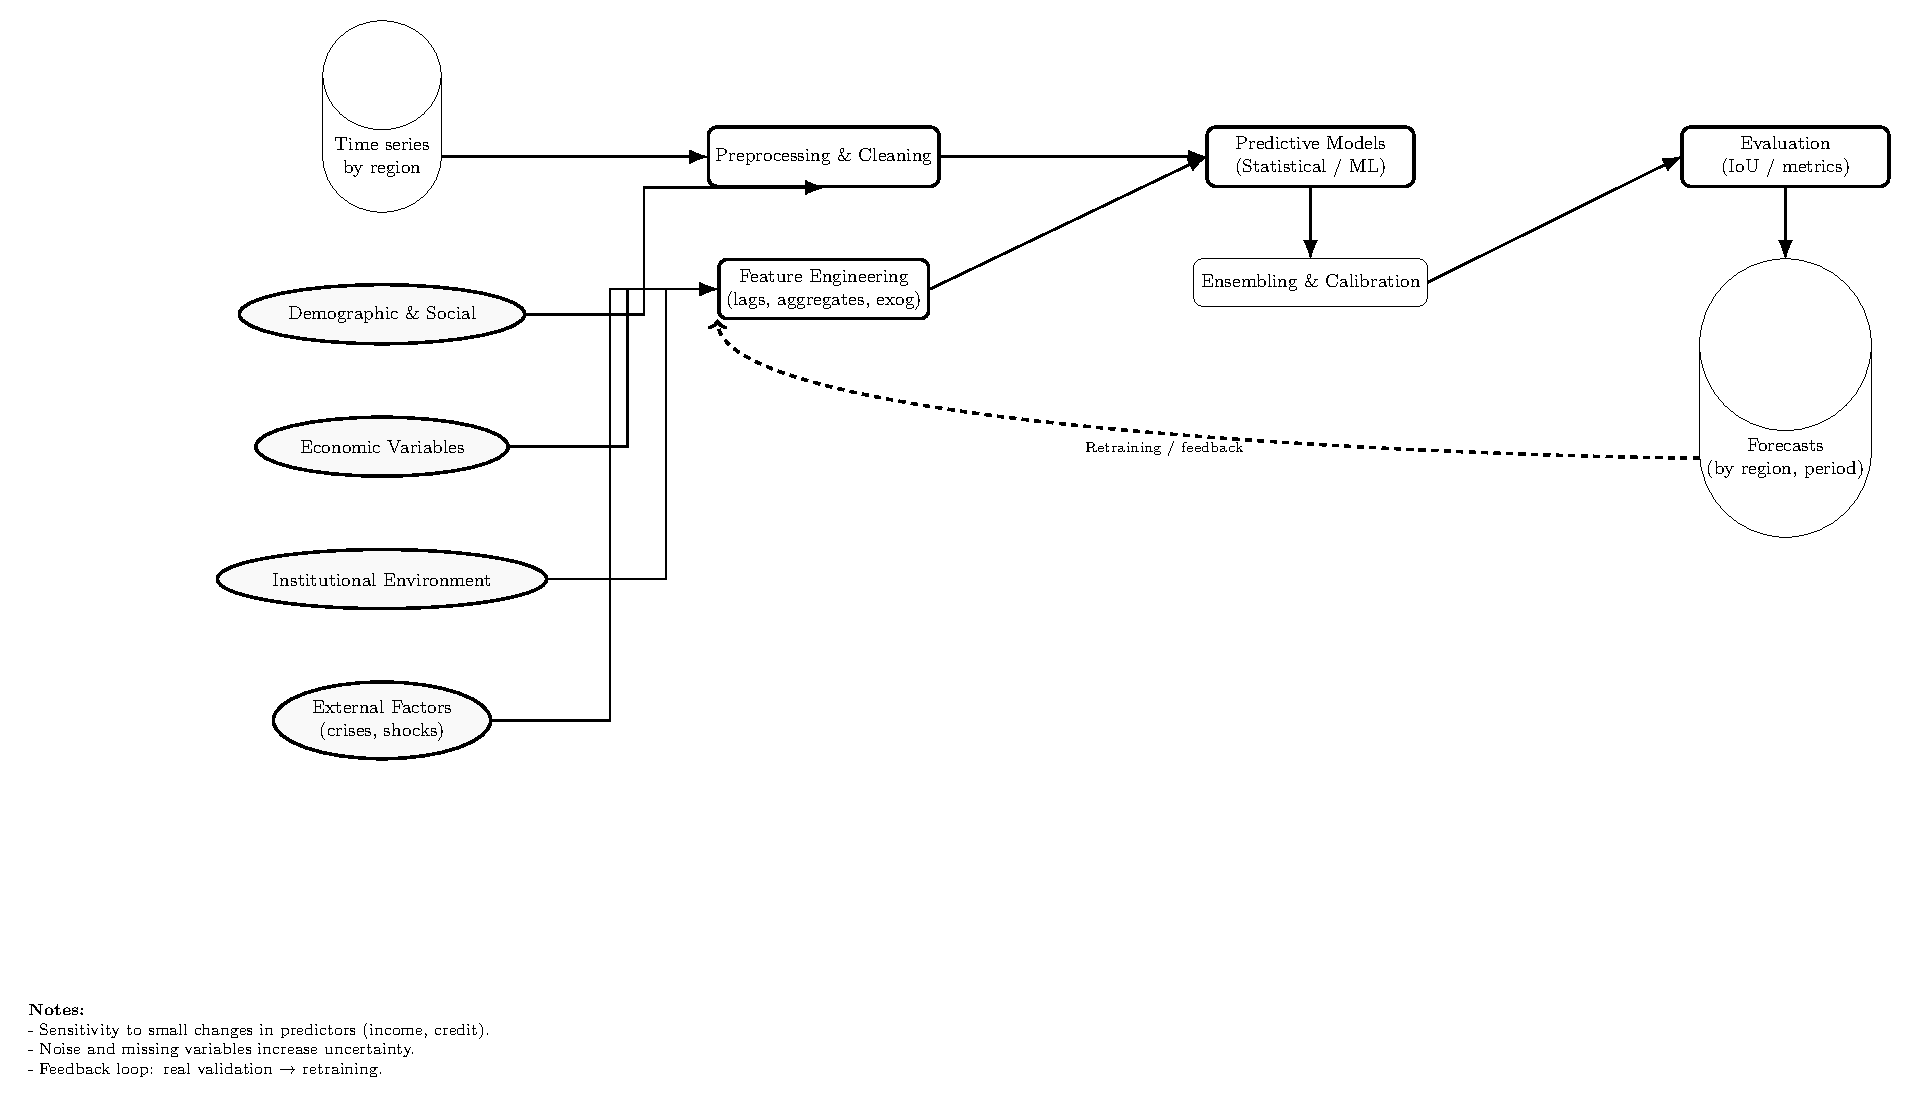
\includegraphics[width=0.48\textwidth]{diagramas (1).pdf}
    \caption{Systemic workflow for microbusiness density forecasting: from raw time series and socio-economic variables to forecasts and retraining.}
    \label{fig:system_workflow}
\end{figure}

\subsection{Complexity and Sensitivity}
The system exhibits the following characteristics:
\begin{itemize}[noitemsep]
    \item \textbf{Complexity:} multicausality, nonlinearity, cumulative effects, high dimensionality, and uncertainty in the data.
    \item \textbf{Sensitivity:}
    \begin{enumerate}[label=\alph*)]
        \item Small changes in key predictors (income, credit, policies) can strongly alter outcomes.
        \item Hyperparameter tuning significantly affects accuracy and the risk of overfitting.
        \item Input errors propagate and amplify over time in forecasts.
        \item Thresholds exist where minor variations cause disproportionate effects.
    \end{enumerate}
\end{itemize}

\subsection{Chaos and Randomness}
A parallel example is the \textit{Google Research – Identify Contrails} competition, linked to atmospheric systems:
\begin{itemize}[noitemsep]
    \item \textbf{Atmospheric chaos:} small variations in humidity or wind lead to very different outcomes.
    \item \textbf{Randomness in data:} sensor noise and labeling errors add uncertainty.
    \item \textbf{Nonlinear feedback:} contrails may grow into larger cloud systems.
    \item \textbf{Butterfly effect:} flight paths or engine types introduce unpredictable variability.
\end{itemize}
This illustrates that chaos and randomness cannot be eliminated but must be managed through robust modeling.

\section{Conclusion}
The analysis highlights both strengths and weaknesses:
\begin{itemize}[noitemsep]
    \item \textbf{Strengths:} problem relevance, extensive historical data, and a clear evaluation metric (IoU).
    \item \textbf{Weaknesses:} data noise, missing variables, sensitivity to external conditions, and limits imposed by chaotic system behavior.
\end{itemize}

In summary, predicting microbusiness density requires models capable of handling uncertainty, adapting to perturbations, and generalizing beyond the training dataset.

%% ------------ References ------------
\bibliographystyle{IEEEtran}
\begin{thebibliography}{1}
\bibitem{shannon1948}
C. E. Shannon, ``A mathematical theory of communication,'' \textit{Bell System Technical Journal}, vol. 27, no. 3, pp. 379--423, 1948.
\end{thebibliography}

\end{document}
